\documentclass[]{article}
\usepackage{lmodern}
\usepackage{amssymb,amsmath}
\usepackage{ifxetex,ifluatex}
\usepackage{fixltx2e} % provides \textsubscript
\ifnum 0\ifxetex 1\fi\ifluatex 1\fi=0 % if pdftex
  \usepackage[T1]{fontenc}
  \usepackage[utf8]{inputenc}
\else % if luatex or xelatex
  \ifxetex
    \usepackage{mathspec}
  \else
    \usepackage{fontspec}
  \fi
  \defaultfontfeatures{Ligatures=TeX,Scale=MatchLowercase}
\fi
% use upquote if available, for straight quotes in verbatim environments
\IfFileExists{upquote.sty}{\usepackage{upquote}}{}
% use microtype if available
\IfFileExists{microtype.sty}{%
\usepackage{microtype}
\UseMicrotypeSet[protrusion]{basicmath} % disable protrusion for tt fonts
}{}
\usepackage[margin=1in]{geometry}
\usepackage{hyperref}
\hypersetup{unicode=true,
            pdftitle={RiskStratifiedEstimation manual},
            pdfauthor={Alexandros Rekkas and Peter R. Rijnbeek},
            pdfborder={0 0 0},
            breaklinks=true}
\urlstyle{same}  % don't use monospace font for urls
\usepackage{color}
\usepackage{fancyvrb}
\newcommand{\VerbBar}{|}
\newcommand{\VERB}{\Verb[commandchars=\\\{\}]}
\DefineVerbatimEnvironment{Highlighting}{Verbatim}{commandchars=\\\{\}}
% Add ',fontsize=\small' for more characters per line
\usepackage{framed}
\definecolor{shadecolor}{RGB}{248,248,248}
\newenvironment{Shaded}{\begin{snugshade}}{\end{snugshade}}
\newcommand{\AlertTok}[1]{\textcolor[rgb]{0.94,0.16,0.16}{#1}}
\newcommand{\AnnotationTok}[1]{\textcolor[rgb]{0.56,0.35,0.01}{\textbf{\textit{#1}}}}
\newcommand{\AttributeTok}[1]{\textcolor[rgb]{0.77,0.63,0.00}{#1}}
\newcommand{\BaseNTok}[1]{\textcolor[rgb]{0.00,0.00,0.81}{#1}}
\newcommand{\BuiltInTok}[1]{#1}
\newcommand{\CharTok}[1]{\textcolor[rgb]{0.31,0.60,0.02}{#1}}
\newcommand{\CommentTok}[1]{\textcolor[rgb]{0.56,0.35,0.01}{\textit{#1}}}
\newcommand{\CommentVarTok}[1]{\textcolor[rgb]{0.56,0.35,0.01}{\textbf{\textit{#1}}}}
\newcommand{\ConstantTok}[1]{\textcolor[rgb]{0.00,0.00,0.00}{#1}}
\newcommand{\ControlFlowTok}[1]{\textcolor[rgb]{0.13,0.29,0.53}{\textbf{#1}}}
\newcommand{\DataTypeTok}[1]{\textcolor[rgb]{0.13,0.29,0.53}{#1}}
\newcommand{\DecValTok}[1]{\textcolor[rgb]{0.00,0.00,0.81}{#1}}
\newcommand{\DocumentationTok}[1]{\textcolor[rgb]{0.56,0.35,0.01}{\textbf{\textit{#1}}}}
\newcommand{\ErrorTok}[1]{\textcolor[rgb]{0.64,0.00,0.00}{\textbf{#1}}}
\newcommand{\ExtensionTok}[1]{#1}
\newcommand{\FloatTok}[1]{\textcolor[rgb]{0.00,0.00,0.81}{#1}}
\newcommand{\FunctionTok}[1]{\textcolor[rgb]{0.00,0.00,0.00}{#1}}
\newcommand{\ImportTok}[1]{#1}
\newcommand{\InformationTok}[1]{\textcolor[rgb]{0.56,0.35,0.01}{\textbf{\textit{#1}}}}
\newcommand{\KeywordTok}[1]{\textcolor[rgb]{0.13,0.29,0.53}{\textbf{#1}}}
\newcommand{\NormalTok}[1]{#1}
\newcommand{\OperatorTok}[1]{\textcolor[rgb]{0.81,0.36,0.00}{\textbf{#1}}}
\newcommand{\OtherTok}[1]{\textcolor[rgb]{0.56,0.35,0.01}{#1}}
\newcommand{\PreprocessorTok}[1]{\textcolor[rgb]{0.56,0.35,0.01}{\textit{#1}}}
\newcommand{\RegionMarkerTok}[1]{#1}
\newcommand{\SpecialCharTok}[1]{\textcolor[rgb]{0.00,0.00,0.00}{#1}}
\newcommand{\SpecialStringTok}[1]{\textcolor[rgb]{0.31,0.60,0.02}{#1}}
\newcommand{\StringTok}[1]{\textcolor[rgb]{0.31,0.60,0.02}{#1}}
\newcommand{\VariableTok}[1]{\textcolor[rgb]{0.00,0.00,0.00}{#1}}
\newcommand{\VerbatimStringTok}[1]{\textcolor[rgb]{0.31,0.60,0.02}{#1}}
\newcommand{\WarningTok}[1]{\textcolor[rgb]{0.56,0.35,0.01}{\textbf{\textit{#1}}}}
\usepackage{graphicx,grffile}
\makeatletter
\def\maxwidth{\ifdim\Gin@nat@width>\linewidth\linewidth\else\Gin@nat@width\fi}
\def\maxheight{\ifdim\Gin@nat@height>\textheight\textheight\else\Gin@nat@height\fi}
\makeatother
% Scale images if necessary, so that they will not overflow the page
% margins by default, and it is still possible to overwrite the defaults
% using explicit options in \includegraphics[width, height, ...]{}
\setkeys{Gin}{width=\maxwidth,height=\maxheight,keepaspectratio}
\IfFileExists{parskip.sty}{%
\usepackage{parskip}
}{% else
\setlength{\parindent}{0pt}
\setlength{\parskip}{6pt plus 2pt minus 1pt}
}
\setlength{\emergencystretch}{3em}  % prevent overfull lines
\providecommand{\tightlist}{%
  \setlength{\itemsep}{0pt}\setlength{\parskip}{0pt}}
\setcounter{secnumdepth}{5}
% Redefines (sub)paragraphs to behave more like sections
\ifx\paragraph\undefined\else
\let\oldparagraph\paragraph
\renewcommand{\paragraph}[1]{\oldparagraph{#1}\mbox{}}
\fi
\ifx\subparagraph\undefined\else
\let\oldsubparagraph\subparagraph
\renewcommand{\subparagraph}[1]{\oldsubparagraph{#1}\mbox{}}
\fi

%%% Use protect on footnotes to avoid problems with footnotes in titles
\let\rmarkdownfootnote\footnote%
\def\footnote{\protect\rmarkdownfootnote}

%%% Change title format to be more compact
\usepackage{titling}

% Create subtitle command for use in maketitle
\newcommand{\subtitle}[1]{
  \posttitle{
    \begin{center}\large#1\end{center}
    }
}

\setlength{\droptitle}{-2em}

  \title{RiskStratifiedEstimation manual}
    \pretitle{\vspace{\droptitle}\centering\huge}
  \posttitle{\par}
    \author{Alexandros Rekkas and Peter R. Rijnbeek}
    \preauthor{\centering\large\emph}
  \postauthor{\par}
      \predate{\centering\large\emph}
  \postdate{\par}
    \date{2019-07-04}


\begin{document}
\maketitle

{
\setcounter{tocdepth}{2}
\tableofcontents
}
\hypertarget{introduction}{%
\section{Introduction}\label{introduction}}

This vignette describes the application of a risk modeling approach to
predictive heterogeneity of treatment effect (HTE) using the
\texttt{RiskStratifiedEstimation} package. More specifically, this
method involves stratifying the population into strata of predicted risk
and performing comparisons of relative and absolute measures of
treatment effect within these risk strata. Our package combines
functionality of the \texttt{CohortMethod} and the
\texttt{PatientLevelPrediction} packages to perform such a risk
stratified effect estimation (RSEE) analysis. To date, only time to
event response variables are conisdered. We will walk through all the
important steps needed to perform an exemplar study. For the
demonstration we will consider the comparison of coxibs to non-steroidal
anti-inflammatory drugs (NSAIDs) in arthritis patients with established
cardiovascular disease with respect to clinically sigificant
gastrointestinal events (CSGIE). For simplicity we focus only in one
coxib -- celecoxib -- and one non-selective NSAID -- naproxen.

\hypertarget{installation-instructions}{%
\section{Installation instructions}\label{installation-instructions}}

\hypertarget{data-extraction}{%
\section{Data extraction}\label{data-extraction}}

\begin{Shaded}
\begin{Highlighting}[]
\NormalTok{connectionDetails <-}\StringTok{ }\NormalTok{DatabaseConnector}\OperatorTok{::}\KeywordTok{createConnectionDetails}\NormalTok{(}\DataTypeTok{dbms =} \StringTok{"postgresql"}\NormalTok{,}
                                             \DataTypeTok{server =} \StringTok{"localhost/ohdsi"}\NormalTok{,}
                                             \DataTypeTok{user =} \StringTok{"joe"}\NormalTok{,}
                                             \DataTypeTok{password =} \StringTok{"supersecret"}\NormalTok{)}

\NormalTok{cdmDatabaseSchema <-}\StringTok{ "my_cdm_data"}
\end{Highlighting}
\end{Shaded}

Covariate settings are defined using

\begin{Shaded}
\begin{Highlighting}[]
\NormalTok{covariateSettings <-}
\StringTok{  }\KeywordTok{createCovariateSettings}\NormalTok{(}
    \DataTypeTok{useDemographicsGender =} \OtherTok{TRUE}\NormalTok{,}
    \DataTypeTok{useDemographicsAgeGroup =} \OtherTok{TRUE}\NormalTok{,}
    \DataTypeTok{useDemographicsIndexMonth =} \OtherTok{TRUE}\NormalTok{,}
    \DataTypeTok{useConditionOccurrenceLongTerm =} \OtherTok{TRUE}\NormalTok{,}
    \DataTypeTok{useDrugExposureLongTerm =} \OtherTok{TRUE}\NormalTok{,}
    \DataTypeTok{useProcedureOccurrenceLongTerm =} \OtherTok{TRUE}\NormalTok{,}
    \DataTypeTok{useMeasurementLongTerm =} \OtherTok{TRUE}\NormalTok{,}
    \DataTypeTok{useCharlsonIndex =} \OtherTok{TRUE}\NormalTok{,}
    \DataTypeTok{useDistinctConditionCountLongTerm =} \OtherTok{TRUE}\NormalTok{,}
    \DataTypeTok{useDistinctIngredientCountLongTerm =} \OtherTok{TRUE}\NormalTok{,}
    \DataTypeTok{useDistinctProcedureCountLongTerm =} \OtherTok{TRUE}\NormalTok{,}
    \DataTypeTok{useDistinctMeasurementCountLongTerm =} \OtherTok{TRUE}\NormalTok{,}
    \DataTypeTok{useVisitCountLongTerm =} \OtherTok{TRUE}\NormalTok{,}
    \DataTypeTok{longTermStartDays =} \DecValTok{-365}\NormalTok{,}
    \DataTypeTok{mediumTermStartDays =} \DecValTok{-180}\NormalTok{,}
    \DataTypeTok{shortTermStartDays =} \DecValTok{-30}\NormalTok{,}
    \DataTypeTok{endDays =} \DecValTok{0}\NormalTok{,}
    \DataTypeTok{excludedCovariateConceptIds =} \KeywordTok{list}\NormalTok{(}\DecValTok{1118084}\NormalTok{, }\DecValTok{1115008}\NormalTok{),}
    \DataTypeTok{addDescendantsToExclude =} \OtherTok{TRUE}
\NormalTok{  )}
\end{Highlighting}
\end{Shaded}

There are many parameters, but they are all documented in the
\texttt{CohortMethod} manual. The \texttt{createCovariateSettings}
function is described in the \texttt{FeatureExtraction} package.

\textbf{IMPORTANT:} Make sure to remove the drugs from the covariates in
order to avoid including them in the prediction step. In this case, we
remove the ingredients (1118084 for celecoxib and 1115008 for naproxen)
and all their descendants from the covariate settings.

\begin{Shaded}
\begin{Highlighting}[]
\NormalTok{cohortMethodData <-}\StringTok{ }
\StringTok{  }\KeywordTok{getDbCohortMethodData}\NormalTok{(}\DataTypeTok{connectionDetails =}\NormalTok{ connectionDetails,}
                        \DataTypeTok{cdmDatabaseSchema =}\NormalTok{ cdmDatabaseSchema,}
                        \DataTypeTok{oracleTempSchema =} \OtherTok{NULL}\NormalTok{,}
                        \DataTypeTok{targetId =} \DecValTok{5613}\NormalTok{,}
                        \DataTypeTok{comparatorId =} \DecValTok{5614}\NormalTok{,}
                        \DataTypeTok{outcomeIds =} \DecValTok{5622}\NormalTok{,  }
                        \DataTypeTok{studyStartDate =} \StringTok{''}\NormalTok{,}
                        \DataTypeTok{studyEndDate =} \StringTok{''}\NormalTok{,}
                        \DataTypeTok{exposureDatabaseSchema =}\NormalTok{ cdmDatabaseSchema,}
                        \DataTypeTok{exposureTable =} \StringTok{'cohort'}\NormalTok{,}
                        \DataTypeTok{outcomeDatabaseSchema =}\NormalTok{ cdmDatabaseSchema,}
                        \DataTypeTok{outcomeTable =} \StringTok{'cohort'}\NormalTok{,}
                        \DataTypeTok{cdmVersion =} \StringTok{'5'}\NormalTok{,}
                        \DataTypeTok{excludeDrugsFromCovariates =} \OtherTok{FALSE}\NormalTok{,}
                        \DataTypeTok{firstExposureOnly =} \OtherTok{FALSE}\NormalTok{,}
                        \DataTypeTok{removeDuplicateSubjects =} \OtherTok{TRUE}\NormalTok{,}
                        \DataTypeTok{restrictToCommonPeriod =} \OtherTok{FALSE}\NormalTok{,}
                        \DataTypeTok{washoutPeriod =} \DecValTok{0}\NormalTok{,}
                        \DataTypeTok{covariateSettings =}\NormalTok{ covariateSettings)}
\end{Highlighting}
\end{Shaded}

\hypertarget{define-study-population}{%
\section{Define study population}\label{define-study-population}}

\begin{Shaded}
\begin{Highlighting}[]
\NormalTok{populationCSGIE <-}\StringTok{ }\KeywordTok{createStudyPopulation}\NormalTok{(}\DataTypeTok{cohortMethodData =}\NormalTok{ cohortMethodData,}
                                         \DataTypeTok{outcomeId =} \DecValTok{5622}\NormalTok{,}
                                         \DataTypeTok{firstExposureOnly =} \OtherTok{TRUE}\NormalTok{, }
                                         \DataTypeTok{restrictToCommonPeriod =} \OtherTok{FALSE}\NormalTok{,}
                                         \DataTypeTok{washoutPeriod =} \DecValTok{0}\NormalTok{, }
                                         \DataTypeTok{removeDuplicateSubjects =} \StringTok{'remove all'}\NormalTok{,}
                                         \DataTypeTok{removeSubjectsWithPriorOutcome =} \OtherTok{FALSE}\NormalTok{, }
                                         \DataTypeTok{riskWindowEnd =} \DecValTok{30}\NormalTok{,}
                                         \DataTypeTok{addExposureDaysToEnd =} \OtherTok{TRUE}\NormalTok{, }
                                         \DataTypeTok{minDaysAtRisk =} \DecValTok{1}\NormalTok{)}
\end{Highlighting}
\end{Shaded}

Note that we’ve set \texttt{firstExposureOnly} to TRUE to get only the
first of the recorded exposures. We set \texttt{removeDuplicateSubjects}
to `remove all', and \texttt{washoutPeriod} to zero because we already
filtered on these arguments when using the
\texttt{getDbCohortMethodData} function. During loading we set
\texttt{restrictToCommonPeriod} to FALSE, and we do the same here
because we do not want to force the comparison to restrict only to time
when both drugs are recorded. We specify the outcome ID we will use, and
that people with outcomes prior to the risk window start date will not
be removed. The risk window is defined as starting at the index date
(\texttt{riskWindowStart} = 0 and \texttt{addExposureDaysToStart} =
FALSE), and the risk windows ends 30 days after exposure ends
(\texttt{riskWindowEnd} = 30 and \texttt{addExposureDaysToEnd} = TRUE).
Note that the risk windows are truncated at the end of observation or
the study end date. We also remove subjects who have no time at risk.

\hypertarget{running-an-rsee-analysis}{%
\section{Running an RSEE analysis}\label{running-an-rsee-analysis}}

To run an RSEE analysis two steps need to be performed. First, a
prediction step where the individual patient risks are estimated. These
estimates are used to stratify patients into strata with similar risk.
In the second step, treament effect estimates are calculated within the
risk strata. In our case, these steps are performed by calling the
following function:

\begin{Shaded}
\begin{Highlighting}[]
\NormalTok{modelSettings <-}
\StringTok{  }\NormalTok{PatientLevelPrediction}\OperatorTok{::}\KeywordTok{setLassoLogisticRegression}\NormalTok{(}\DataTypeTok{variance =} \FloatTok{0.01}\NormalTok{,}
                                                     \DataTypeTok{seed =} \OtherTok{NULL}\NormalTok{)}

\NormalTok{result <-}\StringTok{ }\KeywordTok{runRiskStratifiedEstimation}\NormalTok{(}\DataTypeTok{cohortMethodData =}\NormalTok{ cohortMethodData, }
                                      \DataTypeTok{population =}\NormalTok{ populationCSGIE, }
                                      \DataTypeTok{modelSettings =}\NormalTok{ modelSettings,}
                                      \DataTypeTok{nfold =} \DecValTok{10}\NormalTok{,}
                                      \DataTypeTok{testSplit =} \StringTok{'person'}\NormalTok{,}
                                      \DataTypeTok{testFraction =} \FloatTok{0.3}\NormalTok{,}
                                      \DataTypeTok{savePlpPlots =} \OtherTok{TRUE}\NormalTok{,}
                                      \DataTypeTok{save =} \StringTok{'save_folder'}\NormalTok{,}
                                      \DataTypeTok{riskStrata =} \DecValTok{4}\NormalTok{,}
                                      \DataTypeTok{weightsType =} \StringTok{'ATE'}\NormalTok{,}
                                      \DataTypeTok{useStabilizedWeights =} \OtherTok{TRUE}\NormalTok{,}
                                      \DataTypeTok{truncationLevels =} \KeywordTok{c}\NormalTok{(.}\DecValTok{025}\NormalTok{, }\FloatTok{.975}\NormalTok{),}
                                      \DataTypeTok{timePoint =} \DecValTok{365}\NormalTok{,}
                                      \DataTypeTok{psThreads =} \DecValTok{4}\NormalTok{)}
\end{Highlighting}
\end{Shaded}

\hypertarget{prediction-step}{%
\subsection{Prediction step}\label{prediction-step}}

In this section we demonstrate how to tune the
\texttt{runRiskStratifiedEstimation} function to the desired prediction
settings. First, we need to decide which prediction method we are going
to use. In this specific case, we have selected a LASSO logistic
regression approach. However, one can select any of the several other
approaches described in the \texttt{PatientLevelPrediction} package
vignettes. Next, we need to define the number of folds for tuning the
hyperparameters of the prediction algorithm. In our case we have set
this number to 10. Here, we also split the data in a 70\%-30\% split,
where 70\% of the data are used for training the LASSO regression model
and 30\% is used for evaluating its performance. This split is based on
a random selection of patient IDs (\texttt{testSplit} = ``person'').
Finally, one can choose to generate the default plots provided by the
\texttt{PatientLevelPrediction} package. Note that the result of the
RSEE analysis provides the prediction result, allowing for further
processing, after the run is finished. For more information, consult the
\texttt{PatientLevelPrediction}
\href{https://github.com/OHDSI/PatientLevelPrediction}{manual and
vignettes}.

\hypertarget{estimation-step}{%
\subsection{Estimation step}\label{estimation-step}}

In this section we demonstrate the tuning of the estimation step of our
process. Using the risk estimates of the prediction step described
earlier, we can stratify patients into groups based on the quantiles of
the prediction distribution. Here we divide patients into quartiles of
predicted risk (\texttt{riskStrata} = 4). Since treatment assignment is
not random within risk strata, we need to estimate propensity scores and
apply one of the several available methods in the literature to balance
the covariates. To date, only the inverse probability of treatment
weighting approach can be considered in the package. This means that
patients are weighted by the inverse of the probability to receive the
treamtent they actually received. Two weighting schemes are allowed,
i.e. ``ATE'' that allows the estimation of the average treatment effect
and ``ATT'' that allows the estiamtion of the average treatment effect
on the treated. In order to deal with the presence of very large
weights, we allow for stabilization (\texttt{useStabilizedWeights} =
TRUE). Finally, fixed truncation of the weights can be also considered
in order to set an upper and a lower bound to the permitted size of the
weights. We define these bounds using quantiles of the weight
distribution. here, these bouds are the 2.5\% and the 97.5\% quantiles.

As was mentioned earlier, only time to event response data can be
analyzed with the package. We need to define a period of follow-up for
our study, which in this case, this period is one year
(\texttt{timePoint} = 365). The \texttt{runRiskStratifiedEstimation}
function fits a weighted Cox proportional hazards model to generate
unbiased estimates of the hazard ratios within risk strata. It also
generates weighted Kaplan-Meier estimates within risk strata.

We can allow for parallelization of the propensity score estimation,
which tends to be rather slow when the size of the data is large. In
this case we set the threads to 4, one thread for each risk stratum.

Finally, we can save the result of the analysis to a selected folder.
This folder will then include the prediction result, the hazard ratios
within risk strata along with 95\% confidence intervals, the weighted
Kaplan-Meier estimates within risk strata and the propensity scores.

\hypertarget{plots}{%
\section{Plots}\label{plots}}

The \texttt{RiskStratifiedEstimation} package allows for the
construction of several plots. We have already mentioned that we can
obtain the default plots provided from the
\texttt{PatientLevelPrediction} package for model evaulation.
Additionally, we can derive the propensity score diagnostics described
in the \texttt{CohortMethod} package vignette.

\hypertarget{balance-diagnostics}{%
\subsection{Balance diagnostics}\label{balance-diagnostics}}

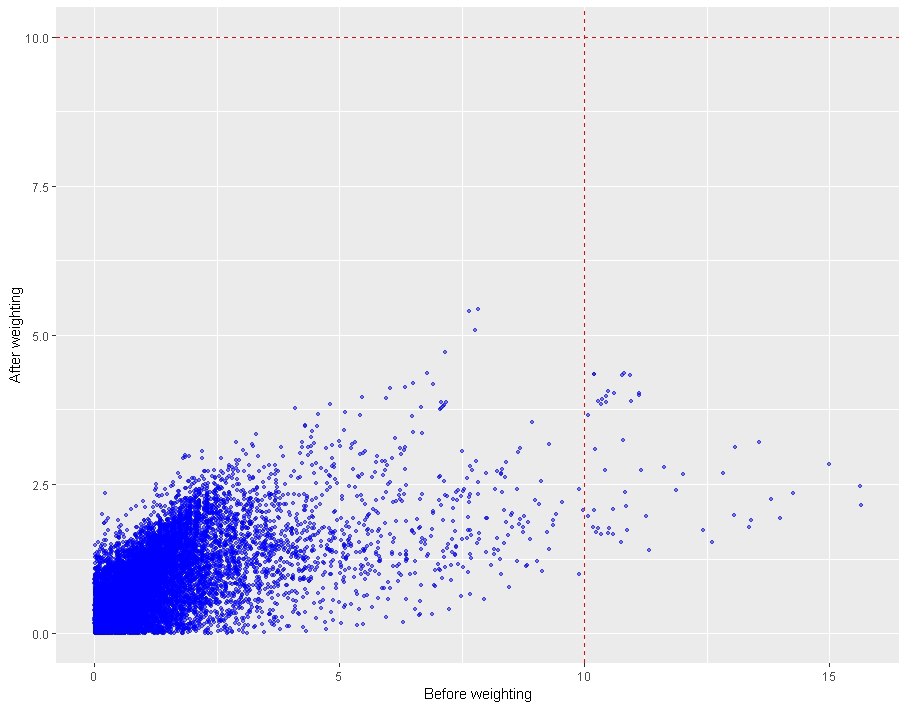
\includegraphics{balancePlot.jpeg} Using the code presented below we can
plot the covariate balance in the weighted population of the 4th
(highest) risk stratum.

\begin{Shaded}
\begin{Highlighting}[]
\KeywordTok{plotCovariateBalance}\NormalTok{(}\DataTypeTok{ps =}\NormalTok{ result}\OperatorTok{$}\NormalTok{ps[[}\DecValTok{4}\NormalTok{]],}
                     \DataTypeTok{cohortMethodData =}\NormalTok{ cohortMethodData,}
                     \DataTypeTok{calculateWeights =} \OtherTok{FALSE}\NormalTok{,}
                     \DataTypeTok{showNotBalancedCovariateIds =} \OtherTok{TRUE}\NormalTok{)}
\end{Highlighting}
\end{Shaded}

\hypertarget{weighted-kaplan-meier}{%
\subsection{Weighted Kaplan-Meier}\label{weighted-kaplan-meier}}

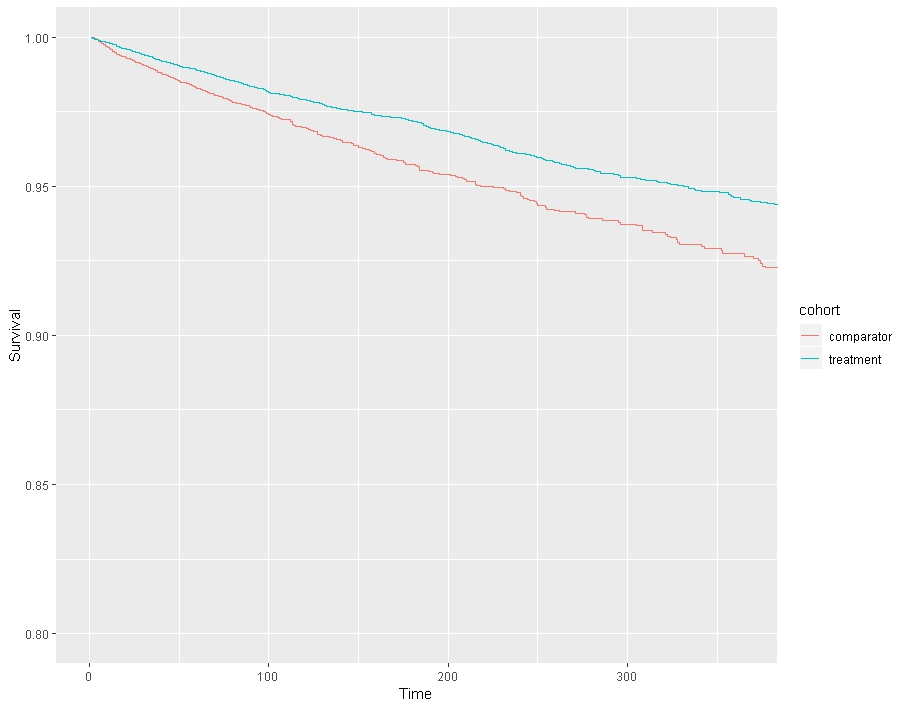
\includegraphics{KMPlot.jpeg} Using the code presented below we can
produce plots of the weighted Kaplan-Meier estimates within risk strata.
The time interval of interest is one year (365 days). Again, we consider
the case of the 4th risk stratum.

\begin{Shaded}
\begin{Highlighting}[]
\KeywordTok{plotWeightedKM}\NormalTok{(}\DataTypeTok{dataKM =}\NormalTok{ result}\OperatorTok{$}\NormalTok{dataKM[[}\DecValTok{4}\NormalTok{]], }
               \DataTypeTok{xlim =} \KeywordTok{c}\NormalTok{(}\DecValTok{0}\NormalTok{, }\DecValTok{365}\NormalTok{), }
               \DataTypeTok{ylim =} \KeywordTok{c}\NormalTok{(.}\DecValTok{7}\NormalTok{, }\DecValTok{1}\NormalTok{),}
               \DataTypeTok{ci =} \OtherTok{FALSE}\NormalTok{)}
\end{Highlighting}
\end{Shaded}

\hypertarget{analysis-result}{%
\subsection{Analysis result}\label{analysis-result}}

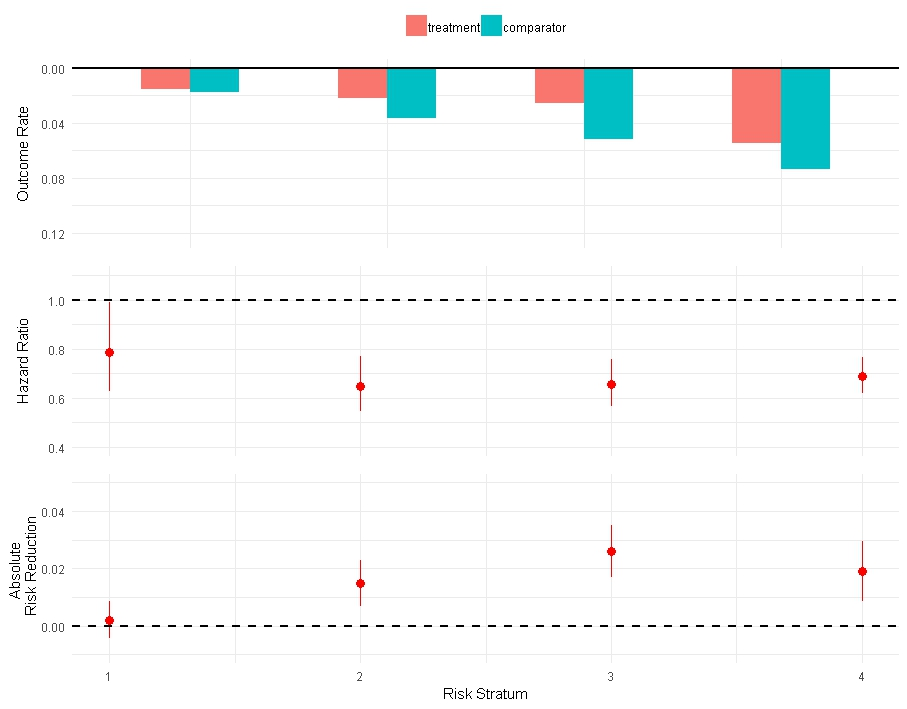
\includegraphics{comparisonPlot.jpeg} Finally, we can produce an
analysis summary plot using the code below. This plot contains the
outcome rates in the propensity weighted populations along with the
absolute and relative (hazard ratios) risk differences.

\begin{Shaded}
\begin{Highlighting}[]
\KeywordTok{comparisonPlot}\NormalTok{(}\DataTypeTok{dataARR =}\NormalTok{ result}\OperatorTok{$}\NormalTok{absoluteRiskReduction, }
               \DataTypeTok{dataRRR =}\NormalTok{ result}\OperatorTok{$}\NormalTok{relativeRiskReduction,}
               \DataTypeTok{cases =}\NormalTok{ result}\OperatorTok{$}\NormalTok{cases,}
               \DataTypeTok{ylimRRR =} \KeywordTok{c}\NormalTok{(.}\DecValTok{4}\NormalTok{, }\FloatTok{1.1}\NormalTok{), }
               \DataTypeTok{ylimARR =} \KeywordTok{c}\NormalTok{(}\OperatorTok{-}\NormalTok{.}\DecValTok{01}\NormalTok{, }\FloatTok{.05}\NormalTok{),}
               \DataTypeTok{ylimCases =} \KeywordTok{c}\NormalTok{(}\DecValTok{0}\NormalTok{, }\FloatTok{.125}\NormalTok{))}
\end{Highlighting}
\end{Shaded}

We can use such a plot to provide insight to the presence of HTE and
draw useful conclusions on treatment assignment.


\end{document}
